\chapter{Design} \label{chapter:design}
This chapter of the report has the purpose of presenting the DC-Net simulator architecture through the utilization of UML diagram notations.

Firstly, I explain the reasons behind my design choices. Secondly, the architecture of the simulator is presented alongside an example of how the event-based communication occurs. Lastly, there is a series of sequence diagrams that exemplifies the data flow between clients and server both for the basic and advanced implementations of the protocol. All of the technologies that happen to be mentioned in this chapter will be presented properly in the implementation section (chapter \ref{chapter:implementation}).


\section{Design Choices}
Throughout the project, I took a number of decisions about the architecture of the simulator. This section justifies these decisions also including which are the original choices proposed by me. 

\subsection{Web Application}
The simulation will be a real-time web-based application that resembles the dynamics of the Dining Cryptographers. I deem choice of a web application appropriate for three reasons:
\begin{enumerate}
    \item From a user perspective, downloading and installing the application and its third-party required components, i.e. dependencies, is likely to end up in technical issues. By using a website, the user can focus on learning the protocol rather than having to overcome possible set-up barriers of a native application;
    \item Building a website entails creating a Graphical User Interface (GUI). This results in a more user-friendly experience in respect to a command line application, which often is the interface of choice for most of the DC-Net simulations available.
    \item A live web application allows clients to connect to the DC-Net server over the Internet. Such distributed architecture is a realistic implementation of the protocol. This differs from available simulations that often emulate all the nodes on the same machine.
\end{enumerate}

\subsection{Network Topology}
The website will employ a client-server architecture. This topology is considered appropriate for the simulation since it offers a farther reach to build complex mechanisms for handling advanced requirements such as multiple rounds of communications or ability to detect message collision.

It is important to highlight that the software implemented is going to be a \emph{simulation}. The role of the server in the application is seen as a facilitator to exchange messages between clients. Therefore, addressing the trust issue mentioned in section \ref{sec:clientserver} is beyond the scope of this project.


\subsection{Key-Exchange Graph Topology}
The key graph employed determines with whom a cryptographer shares secret keys. I chose the ring topology, which entails that a cryptographer is part of two adjacencies, and consequently owns exactly two secret keys each round. 

A full-mesh topology would confer a higher resilience to the network against colluding participants, but it is more complex to implement. Since the addressing the issue of collusion is not part of the requirements, the ring topology was preferred due to its simpler implementation.


\subsection{Original Design Choices: my contributions}
Besides the choices presented above, I propose a number of original features to enhance the usefulness of the protocol in a real-world scenario.







\subsubsection{Three types of rounds (voting, length-calculation, communication)} \label{sec:threeRoundTypes}

Proposals to extend the protocol to multiple rounds of communications in the literature, usually divide communication in a voting phase and a actual sending phase. Although this approach is the same proposed for my implementation, I identified the necessity of a third type of round: length-calculation round. This lead to the choice of splitting the protocol execution in voting, length-calculation and communication rounds. 
The details of each phase is the following:
\begin{enumerate}
    \item \textbf{voting}: participants that would like to send a message try to win the right to do so. Only one user can win a voting round, who becomes the message sender. The key range is simply 0 to 1, where the flipping of one's response is understood as an attempt to win the voting phase. This round type is repeated until a participant want to send a message;
    \item \textbf{length-calculation}: the voting-round winner types the sentence he wants to share anonymously. The message sender will provide this value in the XORed round response. The broadcasted result of this round is therefore the length of the sentence. This information enables the DC-Net service to compute the same number of keys as the length of the sentence before the communication rounds starts. These keys will be delivered in bulk to the participants; The key range chosen for the length-calculation round is 100 to 999. The reason behind this choice is to avoid a scenario in which all randomly generated keys inside the network are very close to 0 and the sentence provided is of greater length. This is likely to reveal the identity of the message sender by simply determining which round response that the server receives is the longest. This round type lasts 10 seconds and can be repeated three times, after which the protocol is aborted.
    \item \textbf{communication}: as many rounds as the message length occur to allow the message sender to anonymously share all characters of the sentence in the form of EASCII codes. The result of this phase will be an anonymously broadcasted sentence into the whole network. The key range is 0 to 255, since the EASCII encoding, explored in the next section, has 256 characters. At the end of this phase, a new voting round starts.
\end{enumerate}


\subsubsection{Extended ASCII encoding interpretation}
To exchange meaningful human-readable messages, I advance the idea of using 8-bit keys during communication rounds and interpret each round result as an Extended ASCII encoded character. 
EASCII encoding is a standard that uses 8 bits (0 to 255) to represent letters, numbers, and symbols.  It is to be noted that regular ASCII has values from 0 to 127 (figure \ref{fig:ascii}), and these are extended with more symbols to 255 in the Extended ASCII version (figure \ref{fig:eascii}). 

\begin{figure}[H]
    \centering
    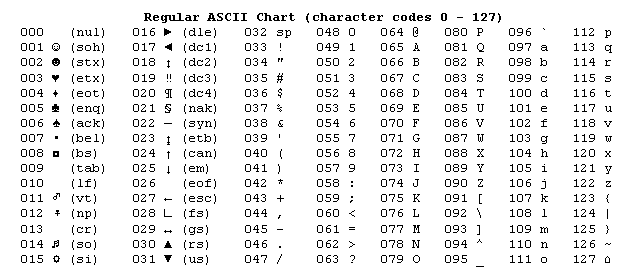
\includegraphics[width=0.7\textwidth]{Images/Design/ascii.png}
    \caption{Regular ASCII Table \cite{Ascii}}
    \label{fig:ascii}
\end{figure}

\begin{figure}[H]
    \centering
    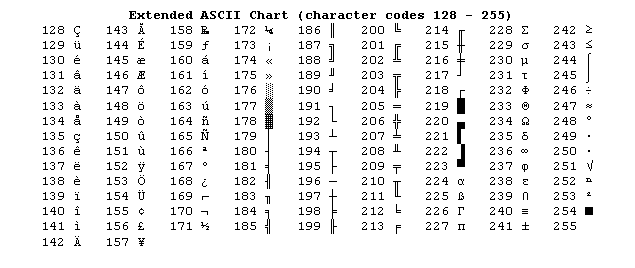
\includegraphics[width=0.8\textwidth]{Images/Design/eascii.png}
    \caption{Extended ASCII Tabled (EASCII) \cite{Ascii}}
    \label{fig:eascii}
\end{figure}


For instance, a participant wishing to send the phrase 'abc' as his sentence, will need three communications rounds to broadcast the whole message. Say that the message sender has 166 and 87 as his secret keys in the first communication round. He will XOR these two values with the number 97, which corresponds to the EASCII character 'a'. This would end up being broadcasted by the server as the final round result. The letter 'b' corresponds to 98 and 'c' is 99, which will be broadcasted anonymously in the two subsequent rounds.


\subsubsection{Collision detection warning} \label{sec:collisionDetectionWarnings}
An important design choice I made, following the implementation of the voting round, is the implementation of a 'message rejected' notification sent by the server to those client who tried to win the voting round but failed. In order words, this is a collision detection mechanism to allow only one winner at a time to transmit a sentence. This workaround has been implemented to avoid the necessity to send a unicast 'success' notification to the winning participant of the voting round, which would obviously uncover who the message sender is to a potential eavesdropper.

In addition, this notification is emitted to the relevant participants only after everyone has provided their voting round responses to the server. This is better than sending such notification immediately back. Otherwise, there exists a scenario in which the first responding client provides his positive intention to send a message, and a second responding client also tries to send a message, but by being rejected immediately, an eavesdropper of the network, would trivially identify the first client as the actual message sender.

For the same reason, if all clients try to send a message in the same round, no matter the timing of the rejection notification,  the sender would be revealed to an eavesdropper by being the only entity not to receive a rejection notification. Hence, if all clients try to send a message in the same round, communication is aborted.


\section{System Architecture}
The architecture of the simulator is simple. There are interaction only between a server, back-end, and a client, front-end. There is no persistent data to be stored in a database (figure \ref{fig:systemArchitecture}).

\begin{figure}[H]
    \centering
    \fbox{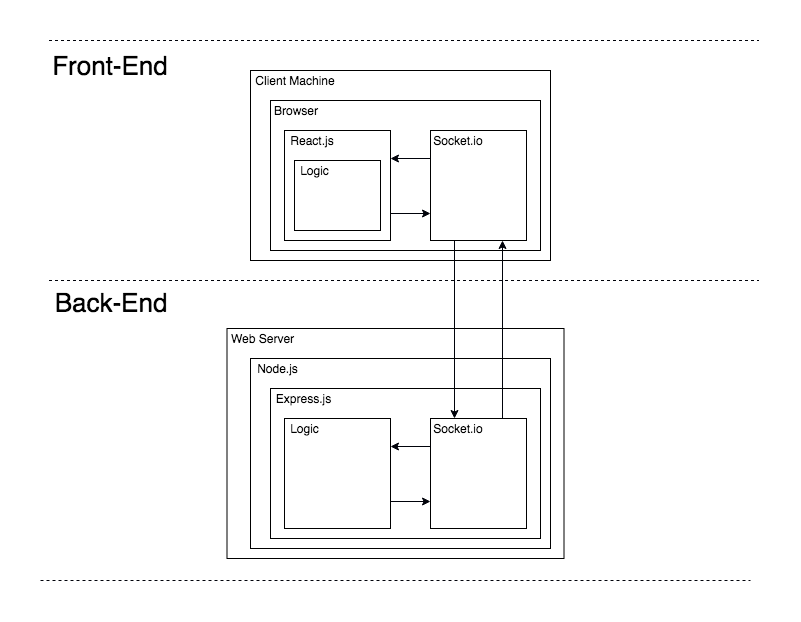
\includegraphics[width=0.9\textwidth]{Images/Design/architecture.png}}
    \caption{System Architecture}
    \label{fig:systemArchitecture}
\end{figure}

The communication between back-end and front-end happens through \lstinline{Socket.io} events. On the server, \lstinline{Socket.io} is attached to the express.js framework. On the client, \lstinline{socket.io} can be found in React.js components.

Both the client and the server will have to perform some logic operations, since what the protocol computes is distributed partially on the clients and partially on the server.

\section{Minimal Distributed Architecture}

As mentioned multiple times, the minimum number of participants to execute the protocol is three. Therefore, this is the same number of clients that needs to establish a connection with the server through \lstinline{socket.io} (figure \ref{fig:distrubtedArchitecture}).

\begin{figure}[H]
    \centering
    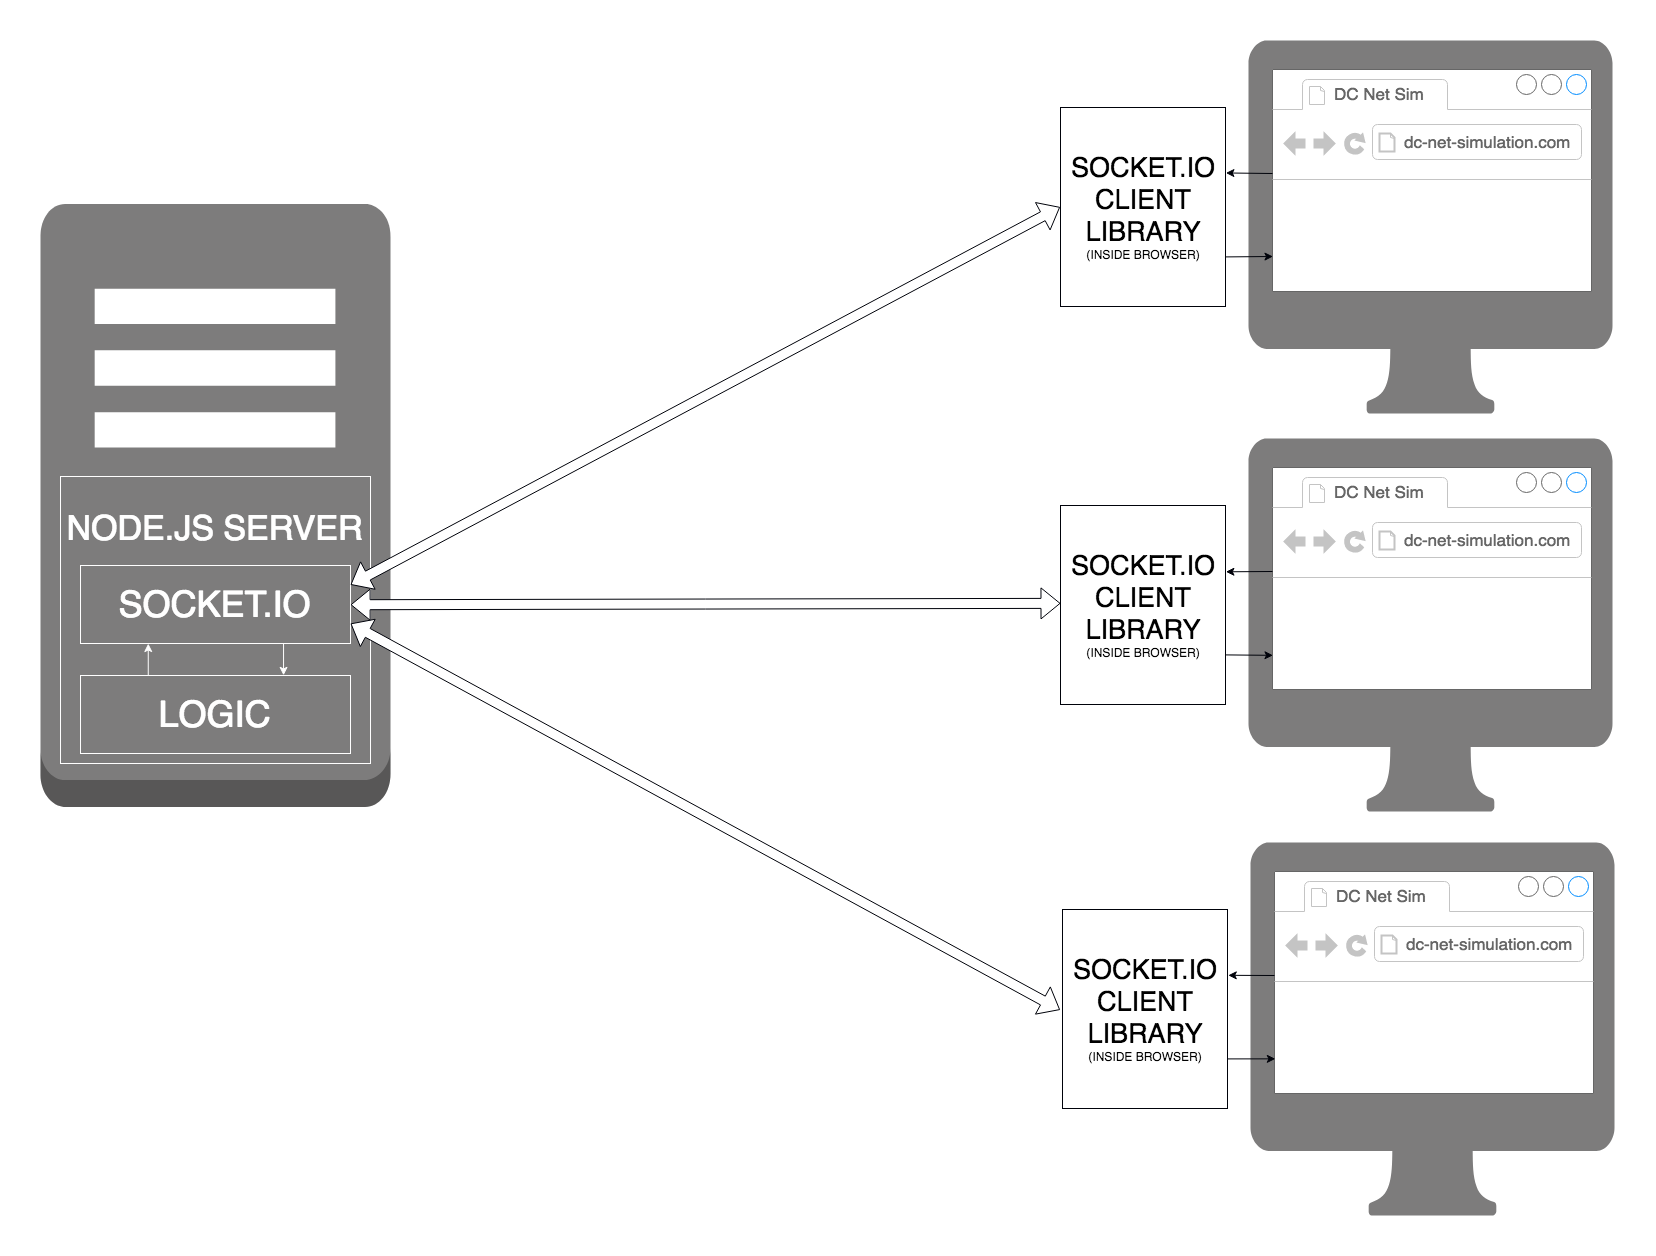
\includegraphics[width=0.8\textwidth]{Images/Design/distributedArchitecture.png}
    \caption{Server with three clients connected}
    \label{fig:distrubtedArchitecture}
\end{figure}

In the final implementation, more than three connections to the server are also supported.

\section{Event-Based Communication Example}
Communication between the cryptographers and DC-Net service is event-based. Therefore, an event needs to be performed by either a client or the server so that a socket event is emitted. If there exists a handler listening to that specific event, a function is invoked. 

\begin{figure}[H]
    \centering
    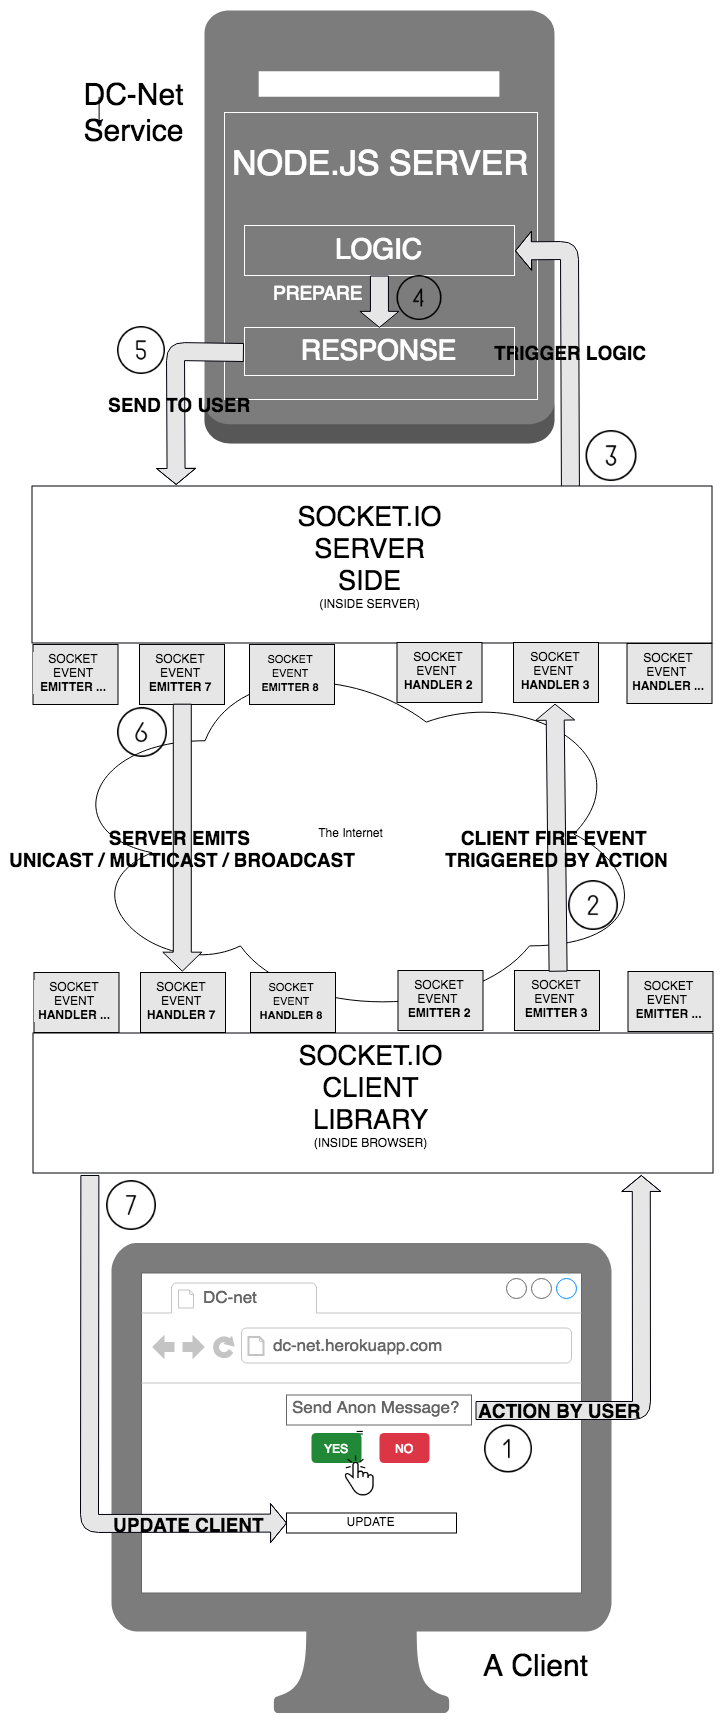
\includegraphics[width=0.55\textwidth]{Images/Design/socketEventEmission.png}
    \caption{Socket event emission from client example}
    \label{fig:socketEventEmission}
\end{figure}

Figure \ref{fig:socketEventEmission} depicts an event being emitted by the client and handled by the server, which in turn emits another event that is handled by the client. The following steps take place:
\begin{enumerate}
    \item a client performs an action;
    \item A socket even is emitted from the client;
    \item The server, who is constantly listening to incoming events, perceived this. The handler is executed, which is supposed to execute some of the protocol logic;
    \item If there exists some response data to be sent back to the client/clients, the response is prepared;
    \item Then the relevant socket event is emitted by the server;
    \item Assuming, that the client possess the relevant handler for the emitted event, a function is triggered;
    \item Lastly, if the information received is a message to be displayed, the client interface is updated.
\end{enumerate}
  

\section{Data flow depiction through sequence diagrams}

The complexity of the Dining Cryptographer is condensed in the exchange of data between clients and server, rather than in the architecture itself. The remaining of the design chapter aims at presenting the most important exchange of messages between clients and server during the protocol execution with sequence diagrams. \newline


\begin{figure}[H]
    \centering
    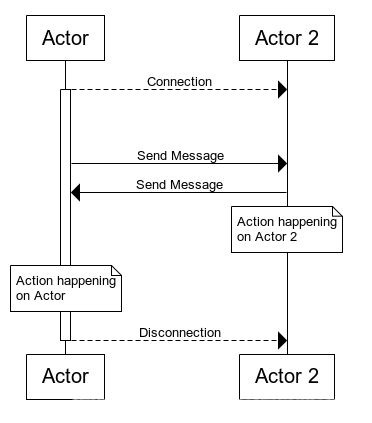
\includegraphics[width=0.5\textwidth]{Images/Design/seqDiagramLegend.png}
    \caption{Sequence Diagram Legend}
    \label{fig:sequenceDiagramLegend}
\end{figure}

Figure \ref{fig:sequenceDiagramLegend} exemplifies the different components that will be found in the upcoming data sequence diagrams: 
\begin{itemize}
    \item an actor can be a client or the server;
    \item a dashed line represents a connection event happening between two actors;
    \item a continuous line is a message or event sent from one actor to the other;
    \item a label over an actor's timeline define an action happening at the physical location of the said actor;
    \item events are chronologically ordered from top to bottom;
\end{itemize}

\subsection{Design of Basic Data Flow}
The basic data flow diagrams explain the flow of data of the core implementation of the protocol achieved.


\begin{figure}[H]
    \centering
    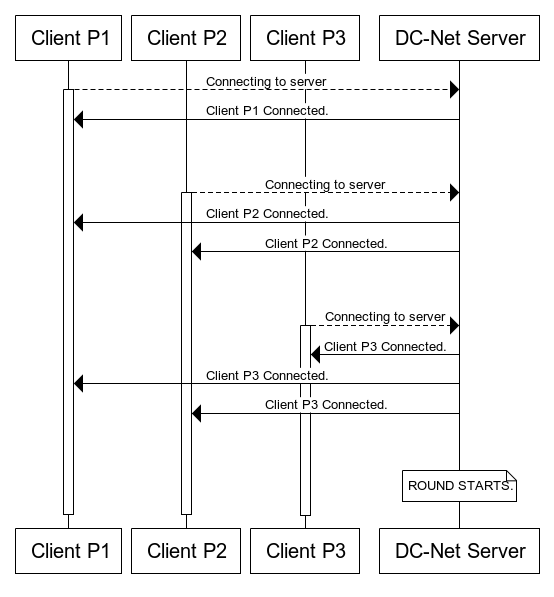
\includegraphics[width=0.7\textwidth]{Images/Design/clientsConnection.png}
    \caption{Connection of three clients needed to start protocol}
    \label{fig:clientsConnection}
\end{figure}


Figure \ref{fig:clientsConnection} shows the connection events of three clients to the server. At each new connection, the server then broadcasts to all participants on the network about the presence of a new participant. Even the connecting client receives the notification of its own connection.

For the sake of brevity, the next diagram will omit the broadcast of the connection event (e.g. 'Client P1 Connected.'), but it is an underlying broadcast that indeed happens.


\begin{figure}[H]
    \centering
    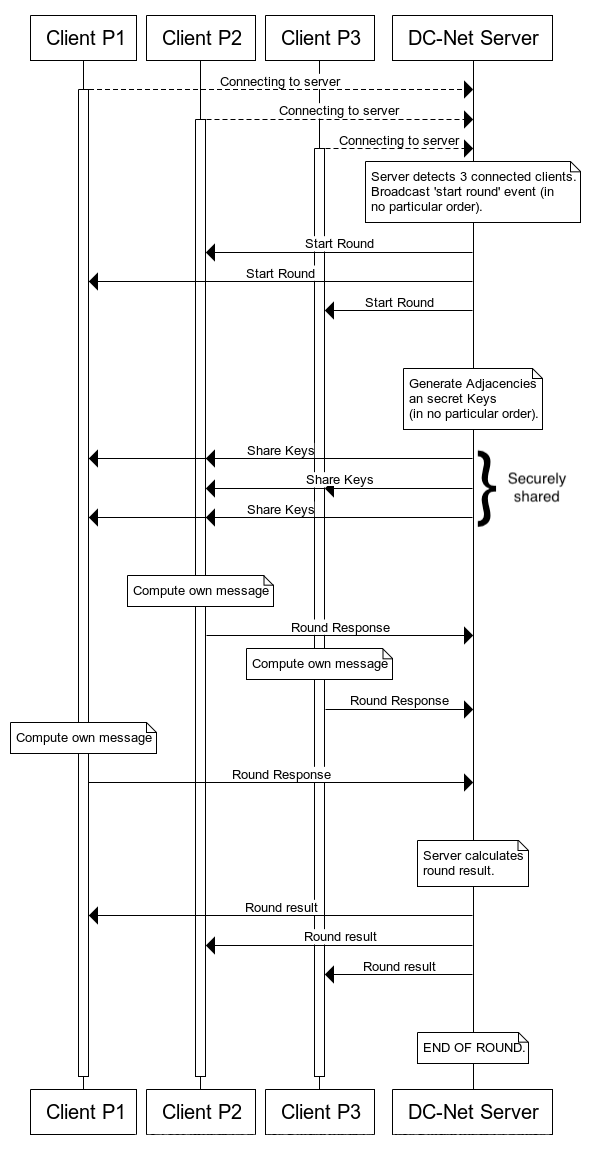
\includegraphics[width=0.6\textwidth]{Images/Design/successfulRound.png}
    \caption{Detailed example of a successful round}
    \label{fig:successfulRound}
\end{figure}

Figure \ref{fig:successfulRound} represents the complete data flow of a successful protocol execution. The steps are the following:
\begin{enumerate}
    \item The DC-Net server listens for incoming connections.
    \item Three clients connect to the server and therefore the server will start the protocol execution;
    \item a start round event is broadcasted by the server, and it reaches all clients in no particular order, who now are aware that the protocol started;
    \item The server generates the adjacency relationship among clients. The key for each adjacency is also generated;
    \item The secret keys are securely shared with each adjacency in the network in particular order;
    \item Each client will decide whether they want to send a message, and once they provide their answer the round response is sent back to the server;
    \item The server detects that all responses have been received and the final round result is calculated;
    \item the round result is broadcasted in no particular order and the protocol execution is completed.
\end{enumerate}

\textbf{It is the presence of step number 6, alongside the XOR of the secret keys, that offers sender anonymity. All participants send a response to the server regardless of whether they are sending a message in their response. Consequently, a sender participant who is actually hiding a message in his response cannot be singled out.}

\begin{figure}[H]
    \centering
    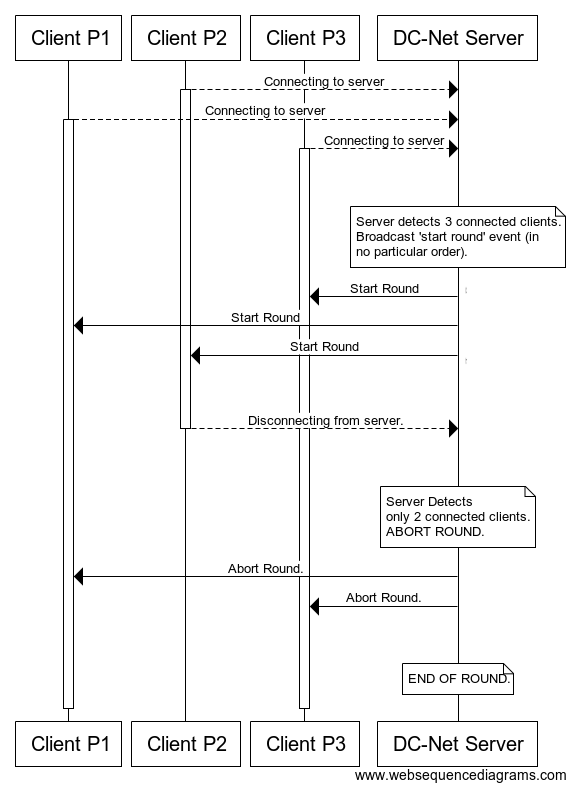
\includegraphics[width=0.7\textwidth]{Images/Design/abortedRound.png}
    \caption{Detailed example of aborted round}
    \label{fig:abortedRound}
\end{figure}

Figure \ref{fig:abortedRound} presents the dynamics of the DC protocol execution that is aborted before completion. Simply put, after the start of the round client P2 disconnects form the server. This event brings the execution to an halt, due to the absence of three participants connected to the server. 


\begin{figure}[H]
    \centering
    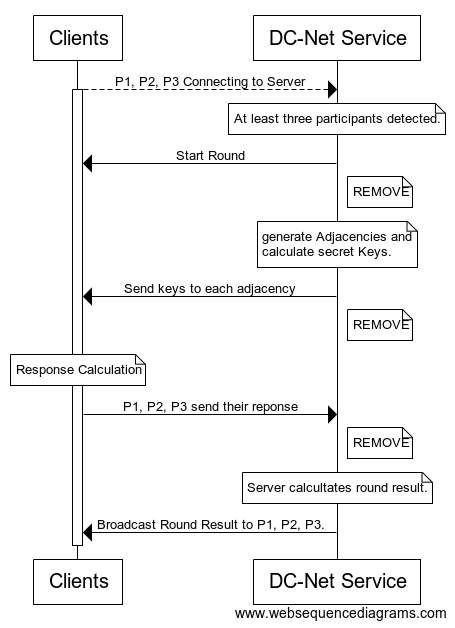
\includegraphics[width=0.7\textwidth]{Images/Design/singleRoundCondensed.png}
    \caption{Concise representation of a single round }
    \label{fig:singleRoundCondensed}
\end{figure}

As we have seen, there is a number of steps involved even in just a single round of communication. To simplify the representation of the following graph with advanced features, a successful protocol execution as represented in figure \ref{fig:successfulRound} can be condensed like in figure \ref{fig:singleRoundCondensed}.



\subsection{Design of Advanced Data Flow}
The advanced data flow diagrams aim at explaining the exchange of data between the client and the server that make use of the advanced features: collision detection, resilient execution with nth participant disconnection during the round, protocol divided in voting, length-calculation and communication round.

\begin{figure}[H]
    \centering
    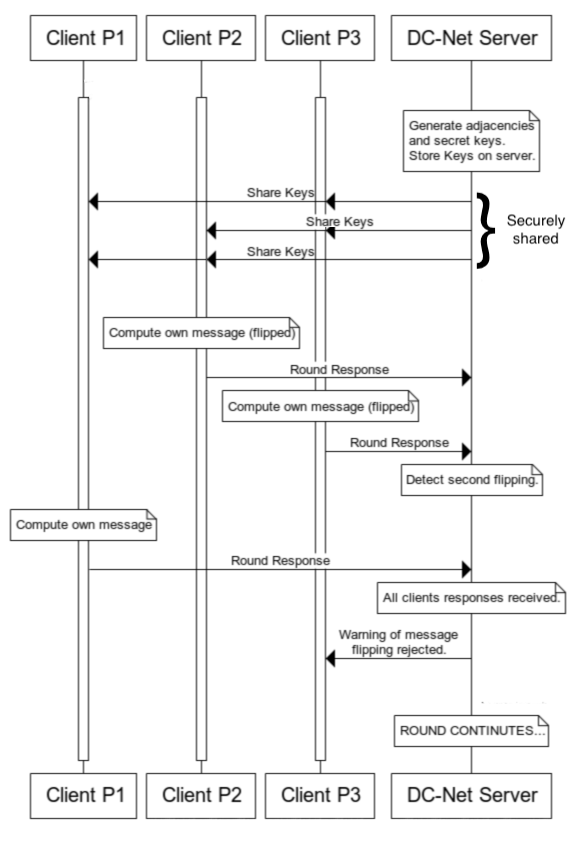
\includegraphics[width=0.6\textwidth]{Images/Design/collisionDetection.png}
    \caption{Detecting message collision}
    \label{fig:collisionDetection}
\end{figure}

\begin{figure}[H]
    \centering
    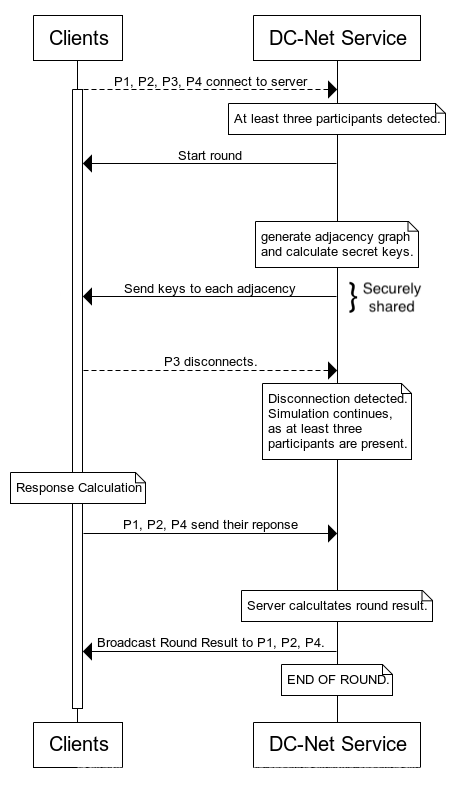
\includegraphics[width=0.5\textwidth]{Images/Design/roundWithDisconnections.png}
    \caption{Round performed with disconnecting client}
    \label{fig:roundWithDisconnections}
\end{figure}

\begin{figure}[H]
    \centering
    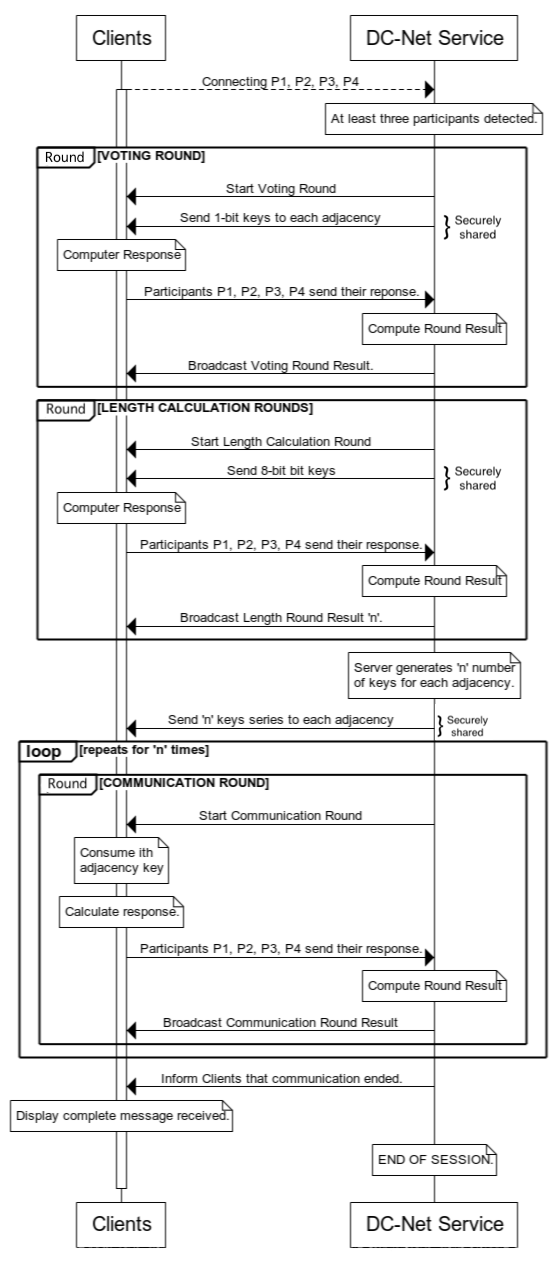
\includegraphics[width=0.6\textwidth]{Images/Design/longRound.png}
    \caption{Representation of complex round of communication}
    \label{fig:longRound}
\end{figure}